% Standalone обёртка для ревью драфта draft_v2.tex.
% Цитаты, перекрёстные ссылки на другие секции и cmd-маркеры заглушены —
% это просто читаемый PDF, не часть диссертационной сборки.
\documentclass[12pt,a4paper]{article}
\usepackage{fontspec}
\setmainfont{Times New Roman}
\setmonofont{Consolas}
\usepackage{polyglossia}
\setdefaultlanguage{russian}
\setotherlanguage{english}
\usepackage[margin=2.2cm]{geometry}
\usepackage{graphicx}
\graphicspath{{../../../}}     % from drafts/ch2/recurrence/ to Disser/
\usepackage{amsmath,amssymb}
\usepackage[dvipsnames]{xcolor}
\usepackage{hyperref}
\hypersetup{colorlinks=true, linkcolor=blue, urlcolor=blue, citecolor=blue}

% Stubs for cross-references and cite commands that won't resolve here
\renewcommand{\cite}[1]{\textcolor{blue!60!black}{[#1]}}
\let\origref\ref
\renewcommand{\ref}[1]{\textcolor{red!70!black}{[\textit{#1}]}}
\providecommand{\link}[1]{}
\providecommand{\future}[1]{}
\providecommand{\source}[1]{}
\providecommand{\TODO}[1]{}

\title{Секция 2.x: метод мультиплексного сетевого анализа коллективной\\
       динамики нейронной активности \\ \large (драфт для ревью)}
\author{}
\date{\today}

\begin{document}
\maketitle

\noindent\textit{Примечание для рецензента: ссылки в квадратных скобках —
\textcolor{blue!60!black}{[Author Year]} — это библиографические цитаты, которые в полной сборке диссертации
оформляются через biblatex (часть из них пока не добавлена в external.bib).
Ссылки на другие секции — \textcolor{red!70!black}{[\textit{sec:...}]} — резолвятся только при сборке всей диссертации.}

\vspace{1em}

% Драфт секции 2.x: Мультиплексный сетевой анализ коллективной динамики
% Подключается в part2.tex вместо текущего \future{}-скелета sec:v2

\section{Метод мультиплексного сетевого анализа коллективной динамики нейронной активности}\label{sec:v2}

Методы оценки эффективной и внутренней размерности (секция~\ref{sec:dim}) описывают коллективную активность как неупорядоченное облако точек в многомерном пространстве. Темпоральная упорядоченность наблюдений при этом не учитывается, хотя сама по себе несёт информацию о динамических режимах популяции. В данной секции описан метод, явно учитывающий темпоральную структуру нейронной активности~--- мультиплексный граф рекуррентности популяции~\cite{Pospelov2024cns}.


\subsection{Метод построения мультиплексного графа рекуррентности}\label{sec:v2_method}

Графы рекуррентности, их количественные характеристики (RQA) и многомерные обобщения рассмотрены в обзоре сетевых методов анализа временных рядов (секция~\ref{sec:network_methods}); там же отмечено, что к сырым сигналам кальциевой флуоресценции \textit{in vivo} метод ранее, по имеющимся данным, не применялся. Ниже описана авторская популяционная конструкция мультиплексного графа рекуррентности и обоснован выбор её параметров для зашумлённых нелинейно-затухающих кальциевых сигналов.

Граф рекуррентности строится для одного временного ряда $x(t)$ через задержечное вложение Такенса~\cite{Takens1981}. Исходный ряд разворачивается в $m$-мерное фазовое пространство: $\mathbf{X}(t) = (x(t), x(t-\tau), \ldots, x(t-(m-1)\tau))$. Элементами графа являются точки $\mathbf{X}(t_i)$; рёбра связывают пары точек, оказавшихся близкими в фазовом пространстве (например, в $k$ ближайших соседях друг друга). Полученная бинарная матрица $R_{ij}$ описывает, в какие пары моментов времени система возвращалась в похожие состояния.

Выбор параметров задержки $\tau$ и размерности вложения $m$ для зашумлённых нелинейно-затухающих сигналов кальциевой флуоресценции требует отдельного обоснования. Временна́я задержка $\tau$ выбиралась как характерное время экспоненциального спада функции временно́й взаимной информации~--- нелинейного аналога автокорреляции; для использованных кальциевых индикаторов (GCaMP6s) это даёт $\tau$ порядка 1~с (медиана по нейронам около 1,2~с), что совпадает с характерным временем отклика индикатора. Размерность вложения $m$ фиксировалась небольшим значением ($m = 2$--$3$): для зашумлённого флуоресцентного сигнала критерий ложных ближайших соседей даёт неустойчиво высокие оценки, тогда как короткое окно вложения $(m-1)\tau$, соизмеримое с длительностью отдельной кальциевой транзиенты, сохраняет локальную геометрию траектории. Робастность результатов к выбору параметров проверялась независимо: качественная картина сохраняется при варьировании $\tau$ в диапазоне характерных времён индикатора и $m \in \{2, 3, 4\}$.

Существующие обобщения метода на несколько временных рядов имеют различную природу. Joint recurrence plot~\cite{Romano2004} строится как поэлементное произведение индивидуальных графов, что соответствует одновременной рекуррентности во всех системах; при $N$ нейронов плотность такой матрицы экспоненциально убывает с ростом $N$. Альтернативой служат мультиплексные сети рекуррентности~\cite{Eroglu2018}, в которых индивидуальные графы трактуются как слои многослойного сетевого объекта. В обоих случаях каждая пара моментов получает либо бинарную оценку (рекуррентны или нет), либо описывается через метрики связности между слоями.

В данной работе для популяции из $N$ нейронов используется иная агрегация~\cite{Pospelov2024cns}. Для каждого нейрона вычисляется индивидуальный граф $R^{(n)}_{ij}$; затем по всем нейронам усредняются их элементы:
\begin{equation}
M_{ij} = \frac{1}{N}\sum_{n=1}^{N} R^{(n)}_{ij}.
\end{equation}
Элементы $M_{ij} \in [0, 1]$ имеют смысл доли нейронов, для которых моменты $t_i$ и $t_j$ являются рекуррентными. В отличие от поэлементного произведения~\cite{Romano2004}, такая агрегация сохраняет полную информацию о доле синхронных рекуррентностей и интерполирует между двумя крайними определениями (одновременная рекуррентность во всех нейронах или хотя бы в одном). В отличие от мультиплексных сетей рекуррентности~\cite{Eroglu2018}, объектом анализа здесь становится единая матрица состояний популяции, к которой можно применять стандартные показатели графов рекуррентности.

\begin{figure}[ht]
\centering
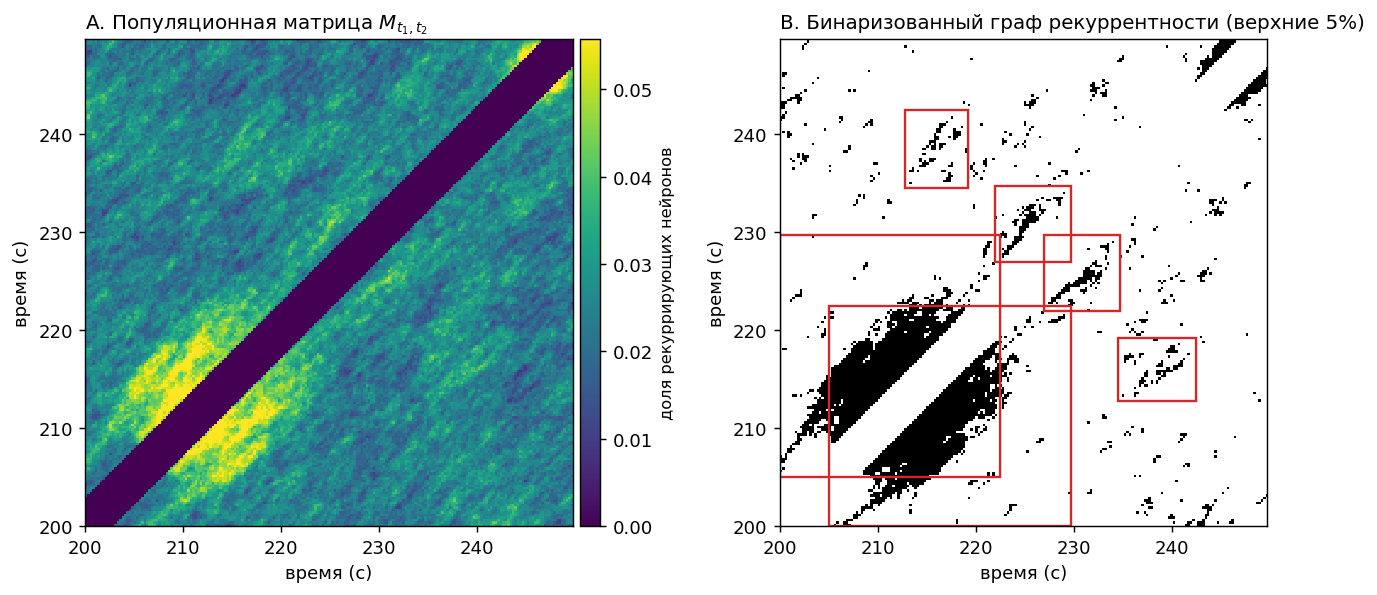
\includegraphics[width=0.92\textwidth]{drafts/ch2/recurrence/results/window_rqa_clustering/fig_method.png}
\caption{Пример мультиплексного графа рекуррентности для 50-секундного фрагмента записи. \textbf{A}~--- континуальная матрица $M_{ij}$; чёрная полоса вдоль диагонали~--- маска близких во времени точек. \textbf{B}~--- бинаризованный граф (порог по 95-му перцентилю недиагональных значений); красными прямоугольниками автоматически выделены внедиагональные блоки рекуррентности.}
\label{fig:rec_method}
\end{figure}

Для последующего анализа матрица $M_{ij}$ бинаризовалась по фиксированному уровню рекуррентности~--- порогу, при котором сохраняется 5\,\% самых больших недиагональных значений. На рис.~\ref{fig:rec_method} приведён пример короткого фрагмента записи: граф содержит не только локальную диагональную рекуррентность, но и дискретные внедиагональные блоки, отражающие повторные посещения одних и тех же коллективных состояний.

Вычисление мультиплексного графа выполнено с помощью пакета DRIADA (секция~\ref{sec:driada}). К получившемуся объекту применяются два независимых дескриптора~--- геометрический (секция~\ref{sec:v2_geometry}) и динамический (секция~\ref{sec:v2_dynamics}), оба основанные на одной и той же матрице $M_{ij}$.


\subsection{Восстановление геометрии среды}\label{sec:v2_geometry}

В секции~\ref{sec:geometry} было показано, что коллективная активность нейронов гиппокампа CA1 при движении по круговой среде укладывается на кольцевое многообразие, изоморфное геометрии трека. Аналогичная гипотеза проверялась здесь для двумерной открытой арены: если близкие в мультиплексном графе моменты времени соответствуют близким положениям животного, то двумерное представление узлов графа должно воспроизводить геометрию арены.

Двумерное представление узлов было получено алгоритмом силового размещения ForceAtlas2~\cite{Jacomy2014}, в котором рёбра графа интерпретируются как пружины с притягивающим действием, а несвязанные пары узлов отталкиваются. Параметры алгоритма были подобраны параметрическим перебором по критерию максимума ранговой корреляции расстояний между точками раскладки и расстояниями между соответствующими положениями животного в арене. Подбор выполнялся однократно на одной репрезентативной сессии, после чего параметры фиксировались и применялись без изменений ко всем 64~сессиям, что исключает их подстройку под отдельные сессии.

Для количественной оценки восстановления использовались четыре показателя. Корреляции Пирсона и Спирмена попарных расстояний в двух пространствах (Мандель-подобные меры) инвариантны к вращению и масштабированию. Procrustes-дисперсия вычислялась после оптимального вращения, отражения и масштабирования раскладки относительно реальной траектории; средняя ошибка восстановления выражалась как RMSE в сантиметрах. Ошибка $k$-NN-декодера ($k = 10$) оценивала возможность предсказать положение животного по точке раскладки: для каждой точки положение предсказывалось как среднее по 10 ближайшим к ней точкам раскладки, и ошибка измерялась в сантиметрах. Эта метрика напрямую сопоставима с физическим размером арены ($44 \times 44$~см).

В качестве контроля использовались перемешанные данные. Чтобы исключить тривиальный эффект разной плотности графа, бинаризация перемешанных матриц проводилась с порогом, обеспечивающим то же число рёбер, что и в реальном графе.

\begin{figure}[ht]
\centering
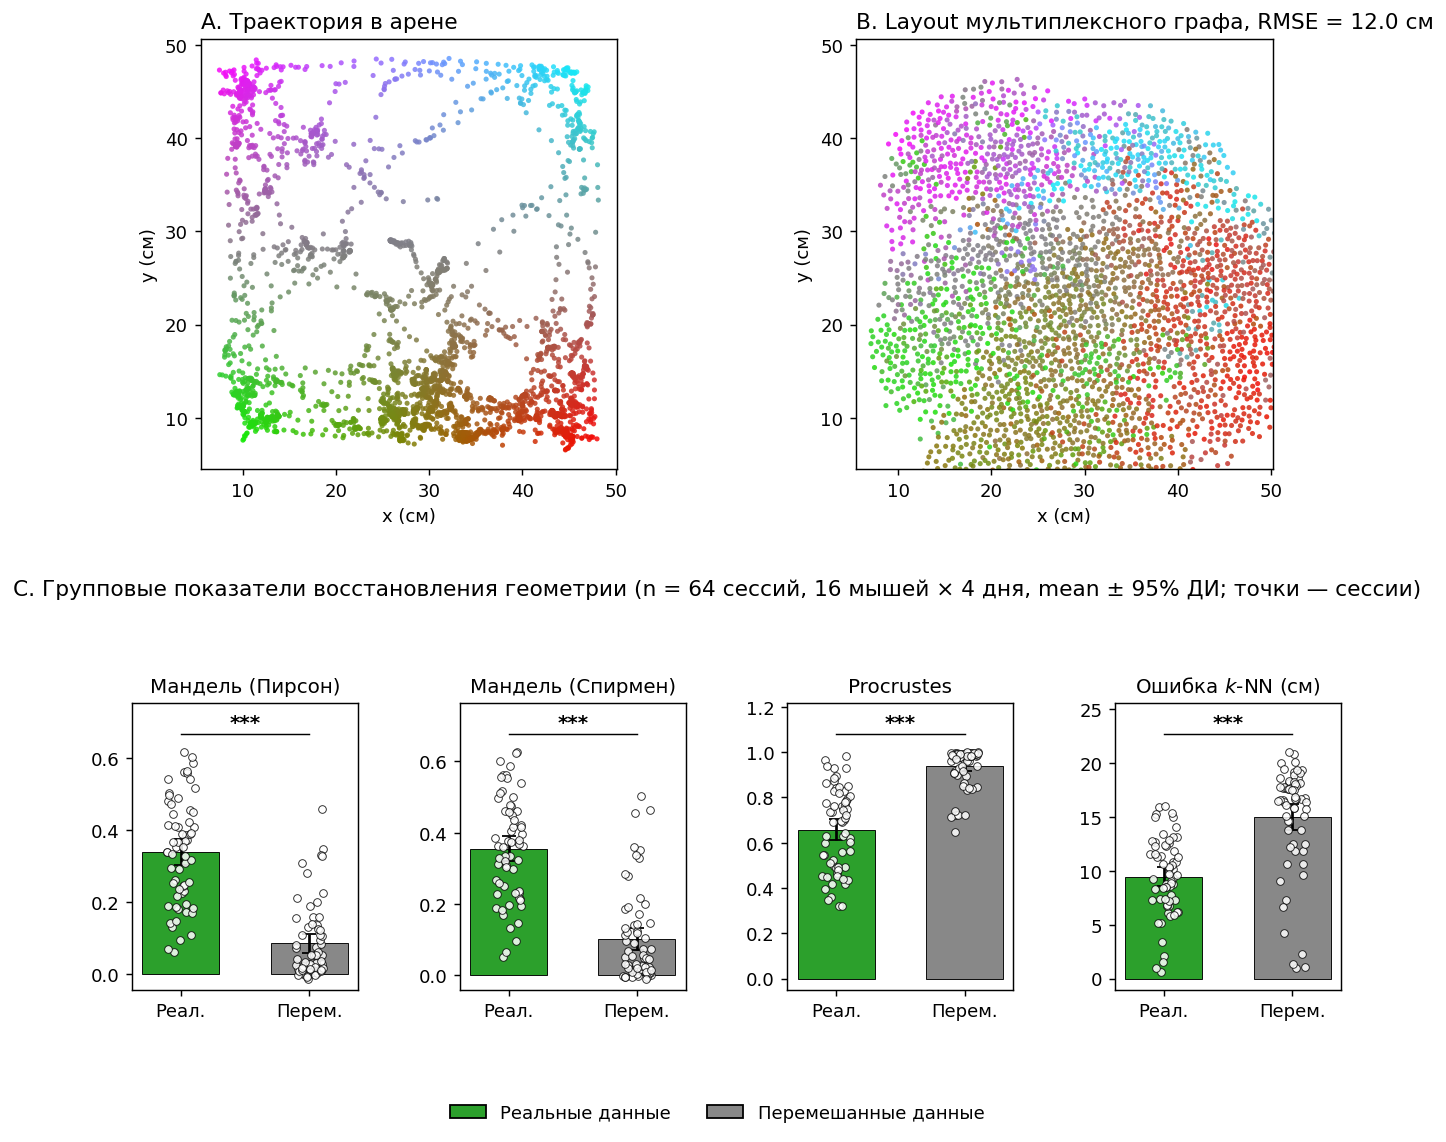
\includegraphics[width=0.95\textwidth]{drafts/ch2/recurrence/results/window_rqa_clustering/fig_geometry.png}
\caption{Восстановление геометрии арены из мультиплексного графа. \textbf{A}~--- траектория животного в одной из сессий, окрашенная двумерной цветовой картой по координатам $(x, y)$. \textbf{B}~--- двумерное представление узлов графа той же сессии после Procrustes-выравнивания относительно траектории, узлы окрашены теми же цветами; RMSE~$= 12{,}0$~см. \textbf{C}~--- групповые показатели восстановления (64 сессии: 16 мышей $\times$ 4 дня; mean $\pm$ 95\,\% ДИ; точки~--- отдельные сессии; серый~--- перемешанные данные с согласованной плотностью графа). Все четыре показателя значимо лучше для реальных данных ($p < 10^{-11}$, критерий Уилкоксона).}
\label{fig:rec_geometry}
\end{figure}

Алгоритм был применён к данным кальциевого имиджинга гиппокампа CA1 при свободном исследовании мышами квадратной арены ($44 \times 44$~см); анализировались 64 сессии (16 мышей, по четыре дня записи; детали эксперимента приведены в секции~\ref{sec:nof_data}). Все четыре показателя восстановления значимо отличались от перемешанных данных (рис.~\ref{fig:rec_geometry}). Медианная ошибка $k$-NN-декодера составила 9{,}5~см при стороне арены 44~см; на перемешанных данных~--- 16{,}6~см, близко к случайному предсказанию. В 63 сессиях из 64 ошибка для реальных данных была меньше, чем для перемешанных ($p = 2 \cdot 10^{-12}$, парный критерий Уилкоксона); медианное улучшение относительно случайного предсказания составило 47\,\%. Медианная корреляция Спирмена расстояний составила 0{,}36 для реальных данных и 0{,}05 для перемешанных; Procrustes-дисперсия~--- 0{,}69 против 0{,}98.

На репрезентативной сессии (рис.~\ref{fig:rec_geometry}A,B) совпадение цветовых градиентов между траекторией в арене и раскладкой графа видно непосредственно: одни и те же области пространства занимают одни и те же области раскладки. Это согласуется с результатом из секции~\ref{sec:geometry} и распространяет его на двумерную геометрию: мультиплексный граф рекуррентности восстанавливает структуру среды и в кольцевом, и в открытом окружении.


\subsection{Динамические режимы коллективной активности}\label{sec:v2_dynamics}

Тот же мультиплексный граф позволяет извлекать темпоральные характеристики динамики. Для каждого скользящего окна длиной 25~секунд внутри графа вычислялся шестимерный вектор количественных характеристик рекуррентности~\cite{Marwan2007}: DET (доля точек на диагональных линиях, характеризует регулярность), LAM (доля точек на вертикальных линиях, характеризует <<застревание>> в близких состояниях), ENTR (энтропия распределения длин линий), TT (среднее время пребывания в одном состоянии), $L_{\text{mean}}$ и $L_{\text{max}}$ (средняя и максимальная длины диагональных линий).

Для проверки наличия структуры в полученных RQA-векторах было применено групповое преобразование главных компонент. Шестимерные векторы со всех 64 сессий и всех окон (всего около 3800 окон) стандартизовались и проецировались на двумерное подпространство наибольшей дисперсии (рис.~\ref{fig:rec_dynamics}A). Первая главная компонента объяснила более 80\,\% дисперсии; шестимерное пространство RQA фактически одномерно. Цветовая раскраска точек по средней скорости движения животного в окне выявила чёткий градиент вдоль первой компоненты: окна с высокой регулярностью соответствуют моментам остановок, окна с низкой регулярностью~--- активному движению. Первая главная компонента имеет содержательную интерпретацию как ось регулярности коллективной динамики.

\begin{figure}[ht]
\centering
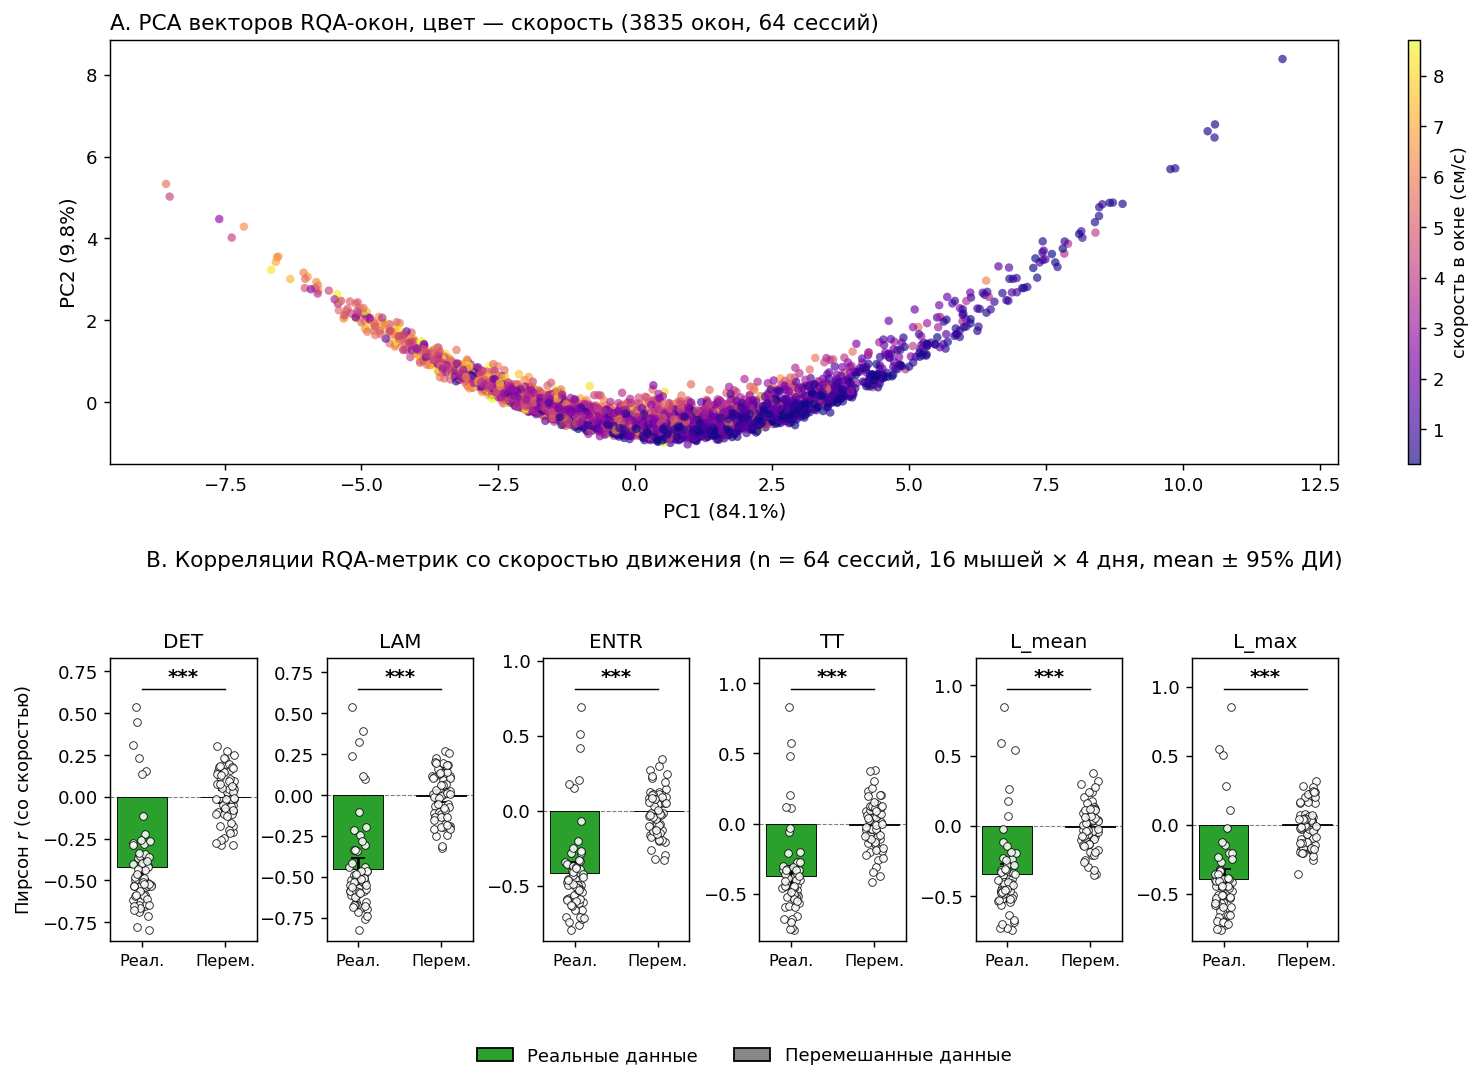
\includegraphics[width=0.95\textwidth]{drafts/ch2/recurrence/results/window_rqa_clustering/fig_dynamics.png}
\caption{Динамические режимы коллективной активности. \textbf{A}~--- двумерное PCA-представление шестимерных RQA-векторов окон по 64 сессиям (около 3800 окон), цвет~--- средняя скорость в окне. Первая главная компонента объясняет большую часть дисперсии и интерпретируется как ось регулярности коллективной динамики. \textbf{B}~--- групповые корреляции каждой RQA-метрики со скоростью; mean $\pm$ 95\,\% ДИ, точки~--- отдельные сессии, серый~--- перемешанные данные. Все шесть характеристик рекуррентности дают согласованную отрицательную корреляцию ($r \approx -0{,}45$, $p < 10^{-8}$).}
\label{fig:rec_dynamics}
\end{figure}

Связь рекуррентных характеристик со скоростью движения проверялась на уровне каждой отдельной метрики (рис.~\ref{fig:rec_dynamics}B). Все шесть характеристик (DET, LAM, ENTR, TT, $L_{\text{mean}}$, $L_{\text{max}}$) дали отрицательную корреляцию со скоростью с медианой группы около $r = -0{,}45$; знак воспроизводится в 58--59 сессиях из 64 для каждой метрики ($p < 10^{-8}$ по критерию Уилкоксона). На перемешанных данных все корреляции близки к нулю. Результат не зависит от выбора одной конкретной характеристики и отражает общее свойство регулярности коллективной траектории.

Полученный режим высокой регулярности при остановках соответствует тому же феномену, который в секции~\ref{sec:dim} был описан через рост эффективной размерности на остановках. Принципиальное различие двух подходов~--- в способе сжатия информации. Эффективная размерность сжимает популяционную активность в скаляр через спектр межнейронной корреляционной матрицы $N \times N$ и несёт только динамическую характеристику. Мультиплексный граф рекуррентности сохраняет всю темпоральную структуру в матрице $T \times T$ и одновременно поддерживает геометрический анализ (секция~\ref{sec:v2_geometry}) и анализ динамических режимов. Эффективная размерность входит в это описание как один из частных дескрипторов, связанный с долей синхронно активных нейронов в данном окне.


\subsection{Обсуждение}\label{sec:v2_discussion}

Предложенный мультиплексный граф рекуррентности обобщает классическую конструкцию графа рекуррентности~\cite{Eckmann1987, Marwan2007} и её многомерные расширения~\cite{Romano2004, Eroglu2018} на популяционный уровень. Результирующее представление коллективной активности~--- взвешенный континуальный объект, а не бинарный, как при попарном joint recurrence~\cite{Romano2004}, и не многослойный, как в мультиплексных сетях рекуррентности~\cite{Eroglu2018}. Это позволяет применять методы теории сетей временных рядов~\cite{Varley2022} непосредственно к данным in vivo кальциевого имиджинга, для которых, по имеющимся данным, подобный анализ ранее не выполнялся.

Среди методов популяционного анализа нейронной активности доминируют модели латентной динамики (GPFA, LFADS, dPCA), извлекающие гладкие низкоразмерные траектории через явные генеративные или вариационные модели, и подходы снижения размерности (PCA, UMAP, Isomap), описывающие коллективную активность как облако точек в подпространстве. Все они оперируют непосредственно на сигналах нейронов и не сохраняют информацию о темпоральной соседности наблюдений в самом представлении. Мультиплексный граф рекуррентности занимает иное место: он работает не с самой активностью, а с её темпоральной структурой возвратов, и для анализа коллективной активности использует методы теории графов и нелинейной динамики, а не вероятностных моделей. Тем самым предложенный метод дополнителен, а не конкурентен по отношению к существующим подходам.

Один и тот же мультиплексный граф даёт две согласованные интерпретации коллективной динамики. Геометрический анализ восстанавливает пространственную карту состояний, и для гиппокампа CA1 она оказывается изоморфной геометрии физической среды. Динамический анализ через RQA-метрики разделяет коллективные режимы по степени регулярности и согласуется с эффективной размерностью (секция~\ref{sec:dim}); в отличие от последней, рекуррентный подход даёт интерпретацию динамики поверх явной геометрии состояний.

Ранний вариант метода был апробирован на данных кругового трека (секция~\ref{sec:geometry}, \cite{Sotskov2022}), где низкоразмерное представление популяционного графа восстанавливало кольцевую геометрию среды (доля объяснённой дисперсии положения $R^2 \approx 0{,}85$), а коллективная траектория совершала переходы между режимами при остановках животного (связь с состоянием движения $R^2 \approx 0{,}73$). На двумерной открытой арене со свободным, нестереотипным поведением восстановление геометрии тем же критерием не достигалось. Настоящая работа решает эту задачу за счёт двух изменений: переход от кластеризации коллективных состояний к прямым мерам восстановления (декодирование положения, корреляция расстояний по Манделю), не требующим дискретной кластерной структуры, и фиксация малой размерности вложения вместо её автоматического подбора. Это позволило воспроизвести восстановление пространственной структуры на 64 сессиях открытого поля (16 мышей, четыре дня записи).

Метод имеет ограничения. Силовое размещение узлов алгоритмом ForceAtlas2 является стохастической процедурой, не оптимизирующей какую-либо явную метрику; альтернативные подходы (UMAP, спектральное вложение) могут давать как лучшие, так и худшие результаты в зависимости от структуры данных, и их сравнительное исследование оставлено для дальнейшей работы. Выбор параметров вложения Такенса для кальциевых данных опирается на эмпирические соображения. Наконец, проанализированные 64 сессии не являются полностью независимыми (по четыре сессии от каждого из 16 животных), поэтому групповые $p$-значения следует трактовать с учётом этой структуры; направленность эффекта тем не менее воспроизводится в подавляющем большинстве отдельных сессий. Анализ изменения восстановленных представлений по мере накопления опыта между днями записи является естественным продолжением.


\end{document}
